\documentclass[11pt,a4paper]{article}

\usepackage[utf8]{inputenc}
\usepackage[T1]{fontenc}
\usepackage[brazilian]{babel}
\usepackage{lmodern}
\usepackage{charter}
\usepackage{indentfirst}
\usepackage{fancyhdr}
\usepackage[margin=2.5cm]{geometry}
\usepackage{graphicx}
\usepackage{float}
\usepackage{caption}
\usepackage{booktabs}
\usepackage{tabularx}
\usepackage{xcolor}
\usepackage{listings}
\usepackage{tikz}
\usetikzlibrary{positioning,arrows.meta}
\usepackage[hidelinks]{hyperref}

\graphicspath{{../img/5g/}}

\definecolor{codebg}{gray}{0.95}
\lstset{
  basicstyle=\ttfamily\small,
  backgroundcolor=\color{codebg},
  frame=single,
  rulecolor=\color{gray!40},
  breaklines=true,
  columns=fullflexible,
  keepspaces=true,
  showstringspaces=false,
  literate={á}{{\'a}}1 {ã}{{\~a}}1 {é}{{\'e}}1 {ç}{{\c{c}}}1 {õ}{{\~o}}1 {ó}{{\'o}}1 {í}{{\'i}}1 {ú}{{\'u}}1 {ê}{{\^e}}1 {à}{{\`a}}1,
}
\lstdefinestyle{yaml}{morecomment=[l]{\#}, commentstyle=\color{gray}\itshape}

\setlength{\headheight}{14pt}
\pagestyle{fancy}
\fancyhf{}
\fancyhead[L]{\small Monitoramento IoT sobre 5G privada}
\fancyhead[R]{\small\nouppercase{\leftmark}}
\fancyfoot[C]{\thepage}
\renewcommand{\headrulewidth}{0.4pt}

\setlength{\emergencystretch}{2em}

\newcommand{\code}[1]{\texttt{#1}}

\title{Monitoramento IoT industrial sobre rede 5G privada\\[0.3em]
  \large Acesso Modbus TCP ao hub IFM e implantação da rede 5G SA}
\author{Miguel Pereira Ramos --- LRC/Unicamp}
\date{\today}

\begin{document}
\maketitle

\section{Objetivo}

Medir a latência de leitura de um sensor industrial (hub IFM IO-Link, Modbus
TCP) através de uma rede 5G \emph{standalone} privada e comparar com o mesmo
sensor acessado por Ethernet. O relatório cobre duas etapas:

\begin{enumerate}
  \item acesso ao hub por Modbus TCP a partir do terminal (validação local);
  \item implantação da rede 5G com rádio real (core Open5GS, gNB srsRAN em
    USRP, roteador HMS como UE) e exposição do hub através dela.
\end{enumerate}

O enlace de rádio é físico. A Figura~\ref{fig:arq} resume a topologia.

\begin{figure}[H]
\centering
\begin{tikzpicture}[
  node distance=0.9cm,
  box/.style={draw, rounded corners, align=center, minimum width=6.2cm, font=\small},
  lbl/.style={font=\footnotesize\itshape, right}]
  \node[box] (hub) {Hub IFM AL1340 (Modbus TCP)\\\code{192.168.10.250:502}};
  \node[box, below=of hub] (ue) {Roteador HMS NV1000 (UE)\\LAN \code{192.168.10.1}};
  \node[box, below=of ue] (gnb) {gNB srsRAN/OCUDU\\USRP B200 / NI-2901};
  \node[box, below=of gnb] (core) {Core Open5GS (AMF, SMF, UPF\ldots)\\host \code{5G-Node-01}};
  \node[box, below=of core] (bench) {\code{bench.py} (medição de latência)};
  \draw[-{Latex}] (hub) -- node[lbl]{Ethernet} (ue);
  \draw[-{Latex}] (ue) -- node[lbl]{RF n78, 20 MHz} (gnb);
  \draw[-{Latex}] (gnb) -- node[lbl]{N2 (NGAP) / N3 (GTP-U)} (core);
  \draw[-{Latex}] (core) -- (bench);
\end{tikzpicture}
\caption{Topologia do experimento.}
\label{fig:arq}
\end{figure}

\section{Materiais}

\begin{table}[H]
\centering
\small
\begin{tabularx}{\textwidth}{@{}lX@{}}
\toprule
Função & Equipamento / software \\
\midrule
Hub & ifm AL1340, mestre IO-Link com interface Modbus TCP~\cite{ifm-al1340,ifm-al1340-manual} \\
Dispositivos IO-Link & Sensor de distância (porta X04) e torre de LED (porta X02) \\
UE & Roteador industrial HMS Anybus NV1000 ``Wireless Router 5G'' (modem 5G, switch de 8 portas)~\cite{hms-nv1000} \\
gNB & OCUDU (srsRAN\_Project)~\cite{srsran} em USRP B200 / NI USRP-2901, driver UHD~\cite{uhd} \\
Core & Open5GS~\cite{open5gs} nativo (systemd) em PC do LRC \\
SIM & Cartão de teste OYEITIMES, gravado com SIM Personalize Tool (Windows 7 + leitor PC/SC) \\
Cliente & Linux; \code{mbpoll}~\cite{mbpoll}, Python com \code{pyModbusTCP}~\cite{pymodbustcp}; simulador com \code{pymodbus}~\cite{pymodbus}; dashboard com Flask-SocketIO~\cite{flask-socketio} \\
\bottomrule
\end{tabularx}
\caption{Hardware e software utilizados.}
\end{table}

\begin{figure}[H]
\centering
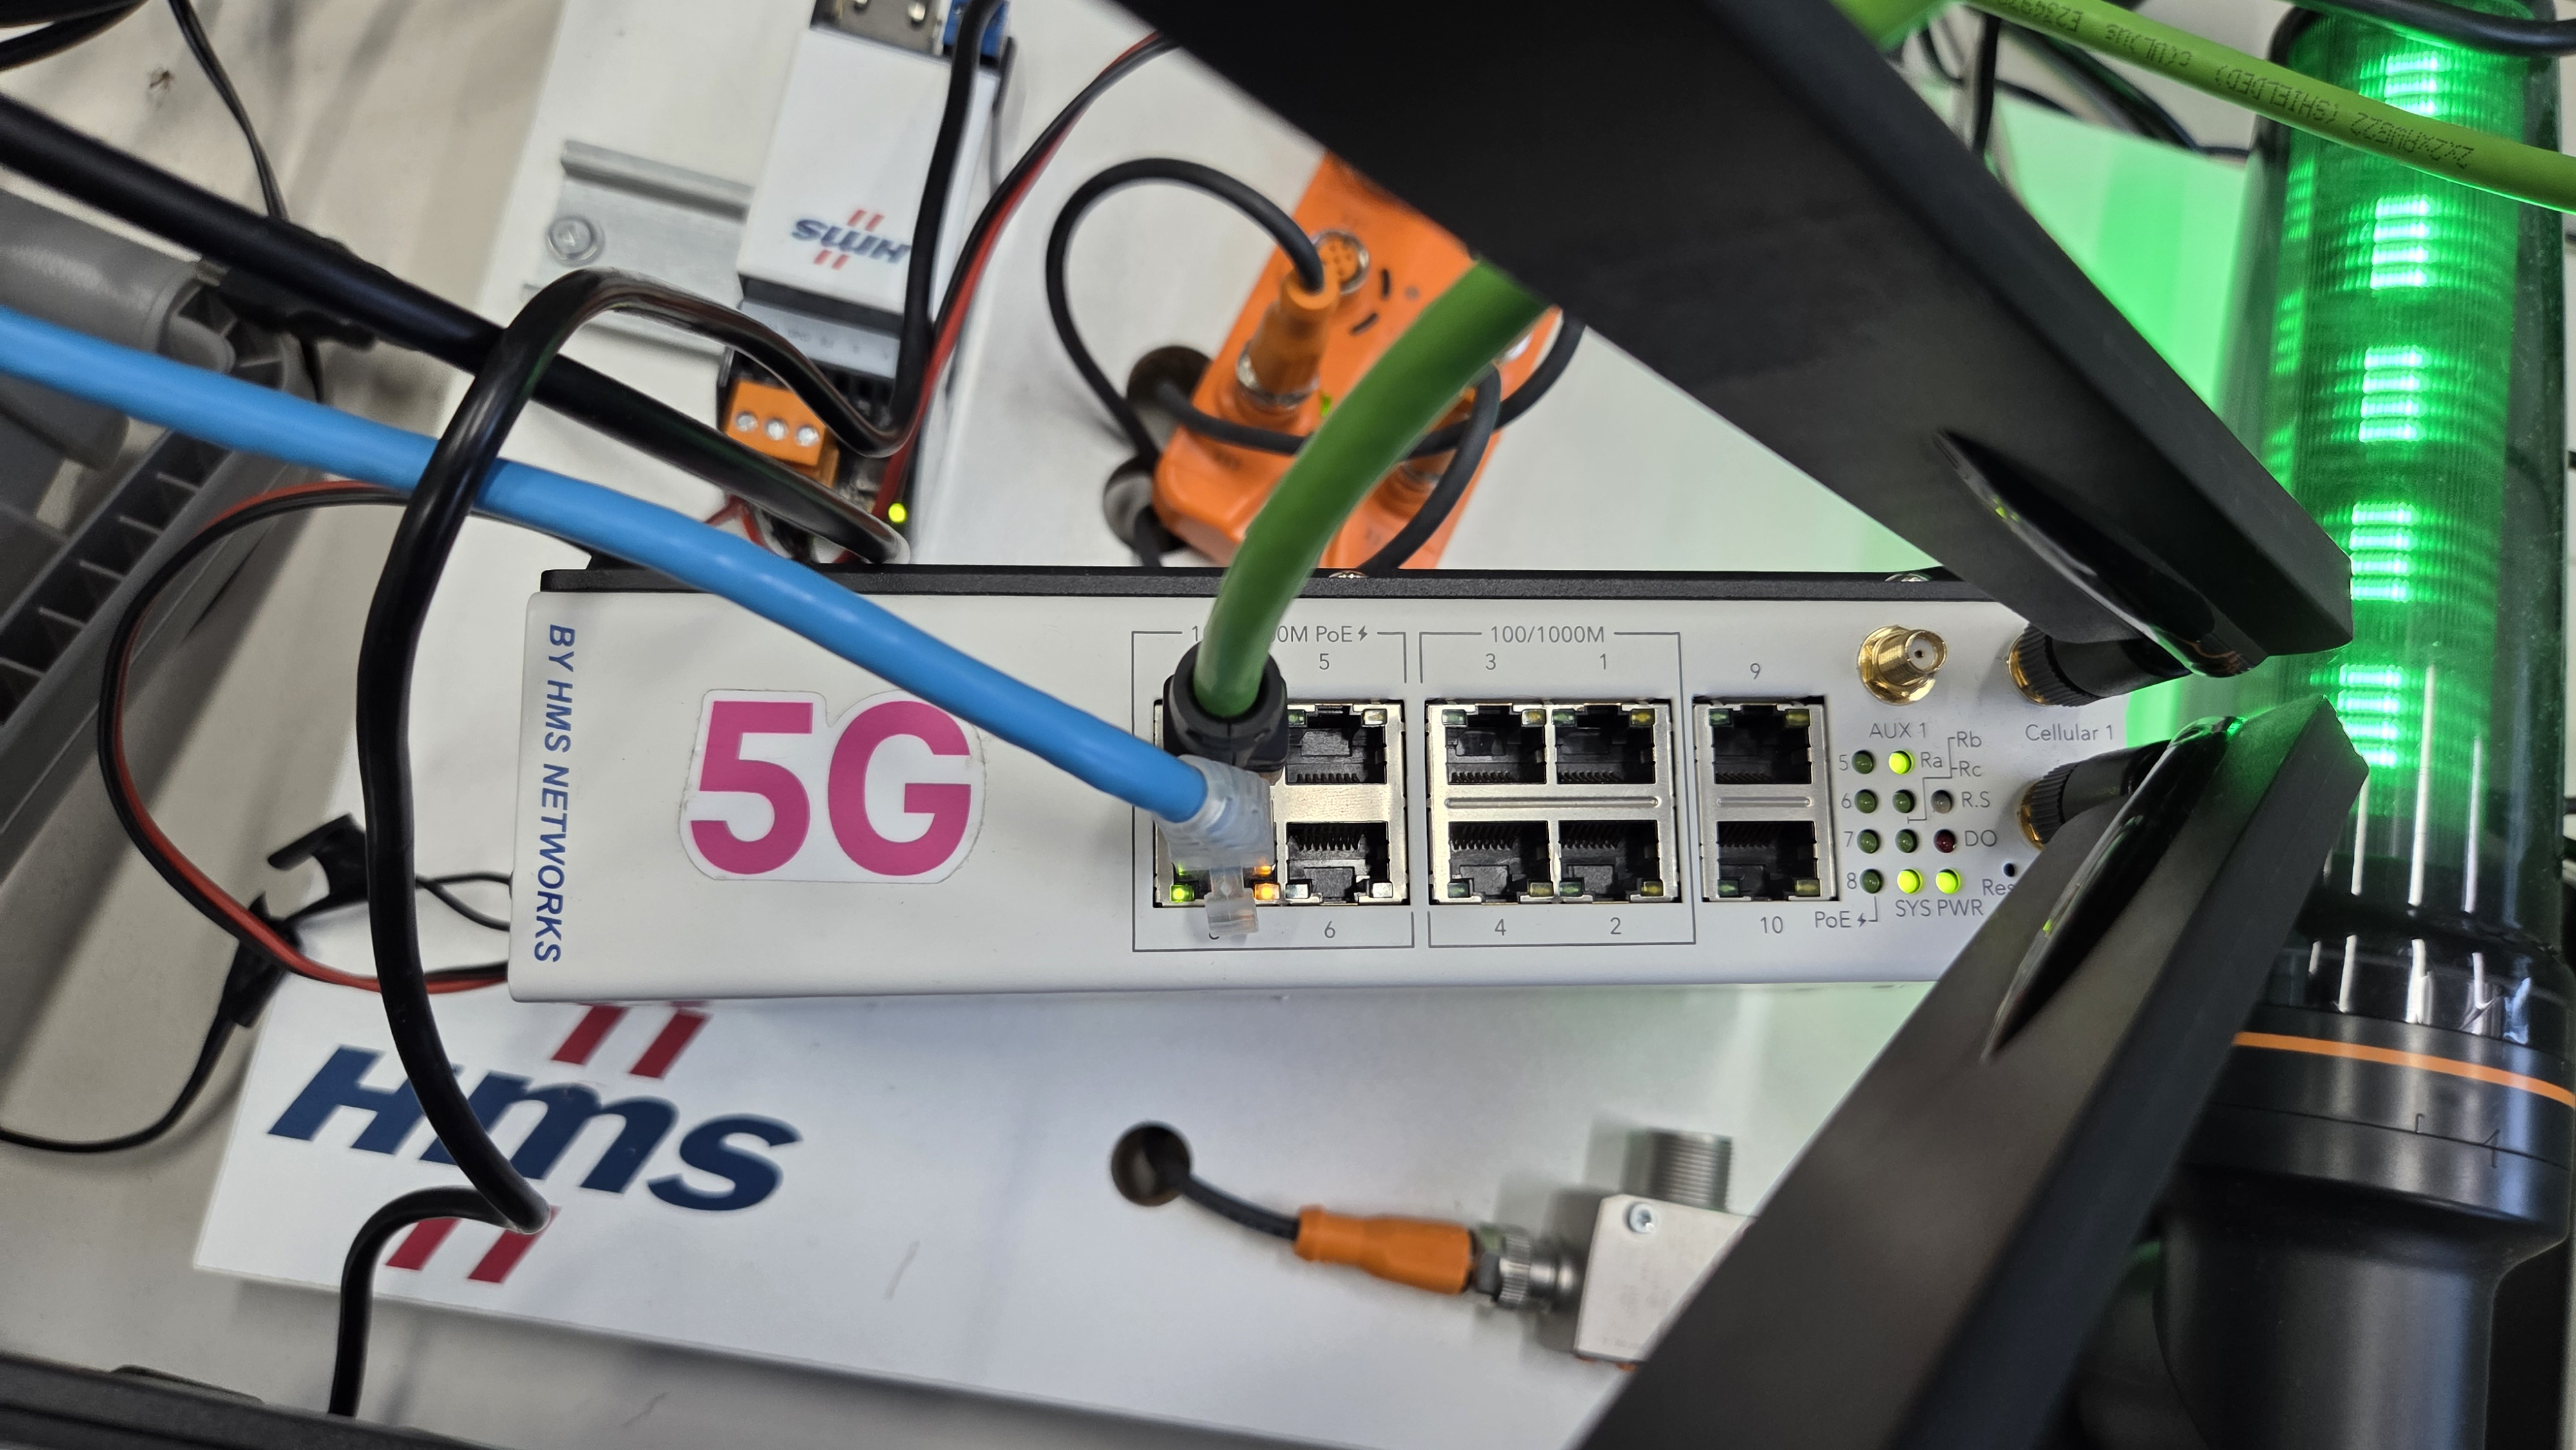
\includegraphics[width=0.6\textwidth]{00-hardware-hms-router.jpg}
\caption{Roteador HMS NV1000 utilizado como UE.}
\end{figure}

\section{Acesso ao hub por Modbus TCP}

O hub responde em \code{192.168.10.250}, porta 502, \emph{unit id} 1.

\subsection{Mapa de registradores do AL1340}

O AL1340 atua como escravo Modbus TCP e expõe configuração, diagnóstico e
dados de processo em \emph{holding registers} de 16 bits~\cite{ifm-al1340-manual}.
Funções suportadas~\cite{modbus}: FC03, FC04, FC06, FC16, FC23 e FC43~\cite[seção 9.3.12]{ifm-al1340-manual}.

\paragraph{Base de endereçamento.} Os números de registrador do manual são
endereços do protocolo (base 0). Ferramentas que usam a notação base 1
(\code{mbpoll}, testadores com prefixo \code{4xxxx}) exigem somar 1: o
registrador 1001 do manual corresponde a \code{401002} nesses
programas~\cite{ifm-modbus-notes}. A biblioteca \code{pyModbusTCP} usa base 0
e recebe o número do manual diretamente.

\paragraph{Acesso por porta.} Na área \emph{Single Port Access}, cada porta
IO-Link ocupa um bloco de 1000 registradores, com a mesma estrutura
(Tabela~\ref{tab:spa})~\cite[seção 13.2.1]{ifm-al1340-manual}. O byte alto
de cada registrador (bits 8--15) vem antes do byte baixo; a inversão é
configurável no registrador 8999 (\emph{Byte Swap}).

\begin{table}[H]
\centering
\small
\begin{tabularx}{\textwidth}{@{}lX@{}}
\toprule
Registrador & Conteúdo (porta X01; X02, X03 e X04 somam 1000, 2000 e 3000) \\
\midrule
1000 & Entradas digitais: pino 2 (byte alto) e pino 4 (byte baixo) \\
1001 & Status da porta (byte alto) e PQI, qualidade dos dados de processo (byte baixo) \\
1002\ldots & Dados de entrada IO-Link ($n$ bytes) \\
1100 & Saída digital do pino 4 \\
1101\ldots & Dados de saída IO-Link ($n$ bytes) \\
\bottomrule
\end{tabularx}
\caption{\emph{Single Port Access} do AL1340 (base 0).}
\label{tab:spa}
\end{table}

O tamanho $n$ dos dados de processo (2, 4, 8, 16 ou 32 bytes por porta) é
definido no registrador 8998. O AL1340 também oferece blocos compactos com os
dados das quatro portas (entrada a partir de 200, saída a partir de 600),
além de diagnóstico (30--69) e configuração (8998--9023). O PQI deve ser
conferido após cada leitura para validar os dados~\cite[seção 9.3.12]{ifm-al1340-manual}.

\paragraph{Registradores usados no projeto.}
\begin{itemize}
  \item \textbf{4002} (\code{mbpoll -r 4003}): primeiro registrador dos dados
    de entrada da porta X04, distância medida pelo sensor em mm.
  \item \textbf{2101--2103} (\code{mbpoll -r 2102}): dados de saída da porta X02,
    6 bytes que definem cor e modo de cada segmento da torre de LED.
    O hub recusa a escrita registrador a registrador (FC06); os três
    registradores são escritos juntos com FC16.
\end{itemize}

\subsection{Conectividade}

\begin{lstlisting}
ping -c 4 192.168.10.250
nc -zv 192.168.10.250 502
\end{lstlisting}

\subsection{Leitura com \code{mbpoll}}

Leitura do sensor (registrador 4002, base 0):

\begin{lstlisting}
mbpoll -m tcp -a 1 -t 4 -r 4003 -c 1 192.168.10.250            # leitura única
mbpoll -m tcp -a 1 -t 4 -r 4003 -c 1 -l 1000 192.168.10.250    # a cada 1 s
mbpoll -m tcp -a 1 -t 4 -r 4001 -c 3 192.168.10.250            # status, PQI e dado
\end{lstlisting}

\begin{table}[H]
\centering
\small
\begin{tabular}{@{}ll@{}}
\toprule
Parâmetro & Significado \\
\midrule
\code{-m tcp} & modo Modbus TCP \\
\code{-a 1} & \emph{unit id} \\
\code{-t 4} & \emph{holding register} (16 bits) \\
\code{-r 4003} & endereço inicial em base 1 (registrador 4002 do manual) \\
\code{-c 1} & número de registradores \\
\code{-l 1000} & intervalo de \emph{polling} em ms \\
\bottomrule
\end{tabular}
\caption{Parâmetros do \code{mbpoll}.}
\end{table}

\subsection{Leitura com Python}

O script \code{ifm\_read.py} do repositório usa \code{pyModbusTCP}; IP,
porta, endereço inicial e quantidade de registradores são definidos no
início do arquivo (\code{ifm\_read.py:6-9}).

\begin{lstlisting}
pip install pyModbusTCP
python3 ifm_read.py
\end{lstlisting}

\subsection{Falhas comuns}

\begin{table}[H]
\centering
\small
\begin{tabularx}{\textwidth}{@{}lXX@{}}
\toprule
Sintoma & Causa provável & Ação \\
\midrule
\code{ping} falha & IP incorreto ou hub fora da rede & Conferir IP no display/app IFM \\
Porta 502 fechada & Modbus TCP desativado ou firewall & Ativar Modbus TCP no hub \\
Falha na leitura & \emph{Unit id} ou endereço inválido & Usar \emph{unit id} 1; variar endereço inicial \\
\emph{Timeout} & Outro cliente Modbus conectado & Encerrar outros clientes (alguns hubs aceitam uma conexão) \\
\bottomrule
\end{tabularx}
\caption{Falhas no acesso Modbus local.}
\end{table}

\section{Rede 5G SA}

\subsection{SIM}

\begin{figure}[H]
\centering
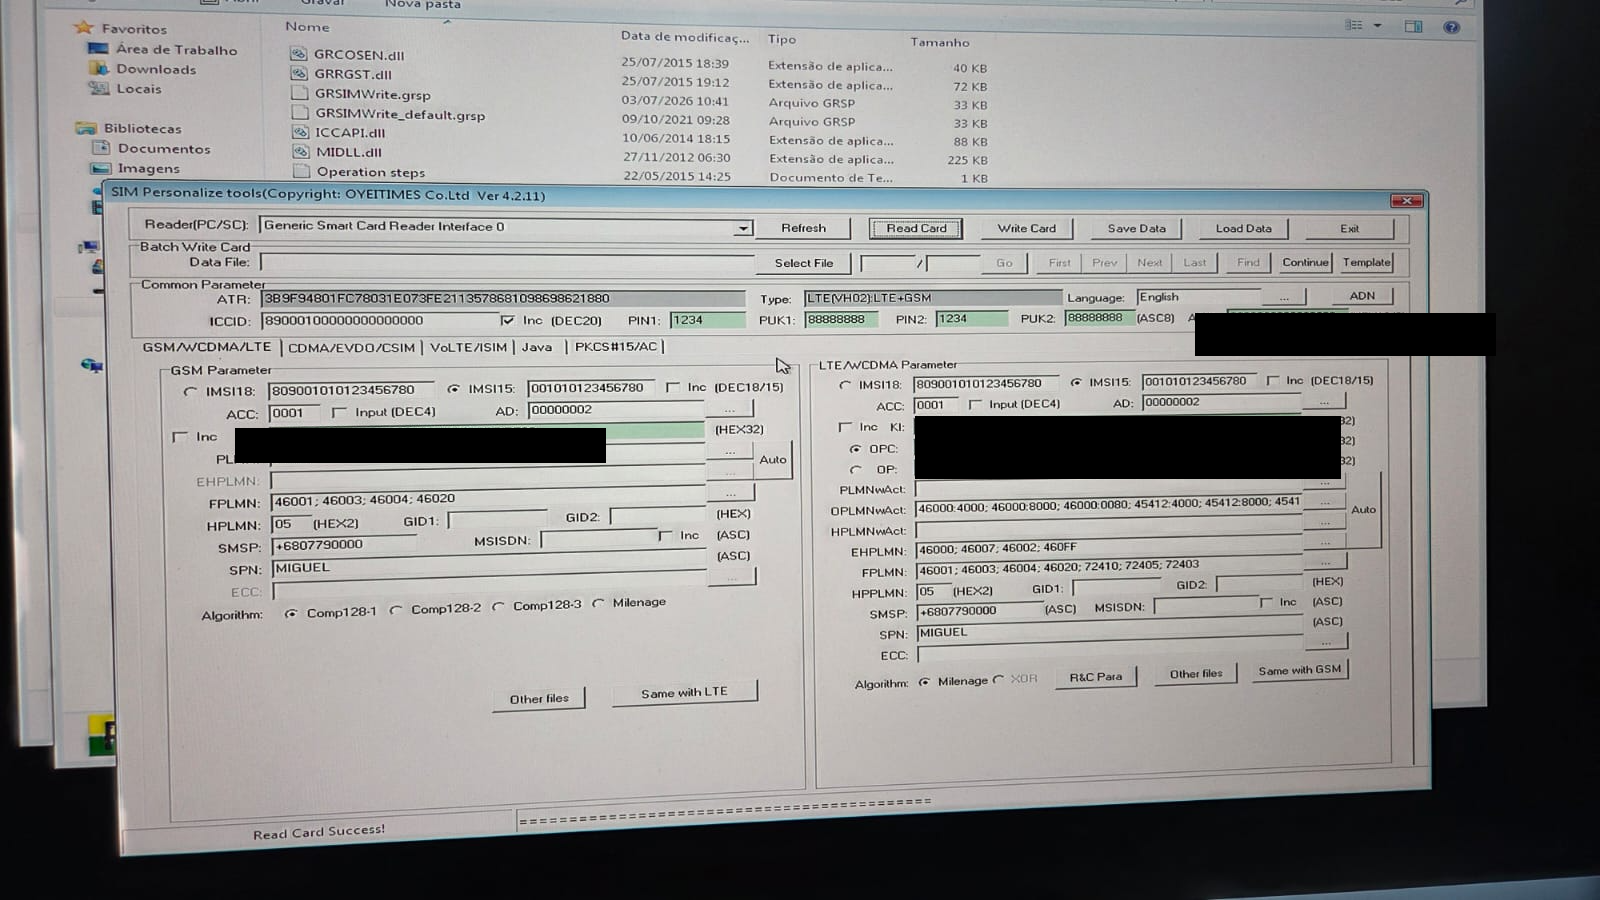
\includegraphics[width=0.75\textwidth]{09-sim-personalize-tool.png}
\caption{SIM Personalize Tool. KI, OPC e ADM ocultados.}
\end{figure}

\begin{itemize}
  \item IMSI \code{001010123456780} (MCC 001, MNC 01); PLMN \code{00101},
    faixa reservada para redes de teste.
  \item Algoritmo Milenage. Ki e OPC gerados na gravação, mantidos fora do
    repositório e reutilizados no cadastro do assinante no core.
\end{itemize}

\subsection{Core Open5GS}

Configuração em \code{/etc/open5gs/*.yaml}. O \code{amf.yaml} original não
tinha bloco \code{ngap}; o AMF não abria a porta 38412 e a gNB falhava com
\code{N2: Failed to connect to AMF ... Connection refused}. Trecho corrigido:

\begin{lstlisting}[style=yaml]
amf:
  sbi:
    server:
      - address: 127.0.0.5
        port: 7777
    client:
      scp:
        - uri: http://127.0.0.200:7777
  ngap:
    server:
      - address: 127.0.0.5      # endereço usado pela gNB
  guami:
    - plmn_id: {mcc: 001, mnc: 01}
      amf_id: {region: 2, set: 1}
  tai:
    - plmn_id: {mcc: 001, mnc: 01}
      tac: 1                    # deve coincidir com o TAC da gNB
  plmn_support:
    - plmn_id: {mcc: 001, mnc: 01}
      s_nssai:
        - sst: 1
\end{lstlisting}

As funções de rede usam comunicação indireta: \code{client.nrf} fica
comentado e todas apontam para o SCP (\code{127.0.0.200:7777}), que encaminha
ao NRF (\code{127.0.0.10:7777}). É o padrão do Open5GS, não um erro.

Assinante cadastrado na WebUI (porta 9999): IMSI acima, Ki/OPC da SIM,
Milenage, \code{sst 1}, DNN \code{internet}.

\subsection{gNB}

Banda n78, 20 MHz, \code{dl\_arfcn 632628} (3489,42 MHz):

\begin{lstlisting}[style=yaml]
cu_cp:
  amf:
    addr: 127.0.0.5
    port: 38412
    bind_addr: 127.0.0.1
    supported_tracking_areas:
      - tac: 1
        plmn_list:
          - plmn: "00101"
            tai_slice_support_list:
              - sst: 1
ru_sdr:
  device_driver: uhd
  device_args: type=b200      # NI-2901 usa o driver b200
  srate: 23.04
  tx_gain: 75
  rx_gain: 75
  otw_format: sc16
  clock_source: internal
  sync_source: internal
cell_cfg:
  dl_arfcn: 632628
  band: 78
  channel_bandwidth_MHz: 20
  common_scs: 30
  plmn: "00101"
  tac: 1
  pci: 1
  nof_antennas_dl: 1
  nof_antennas_ul: 1
\end{lstlisting}

O TAC precisa ser igual em três campos:
\begin{itemize}
  \item \code{cell\_cfg.tac} (gNB);
  \item \code{cu\_cp.amf.supported\_tracking\_areas[].tac} (gNB);
  \item \code{amf.tai.tac} (core).
\end{itemize}
Divergências produziram:

\begin{itemize}
  \item gNB $\neq$ AMF: NG Setup rejeitado com \code{unknown-PLMN-or-SNPN};
  \item divergência interna da gNB: \code{Could not find cell PLMN \allowbreak '00101'
    and cell TAC '1' in the CU-CP supported tracking areas list}.
\end{itemize}

A taxa de 23,04~MSps exige USB~3. Em USB~2 o UHD emite
\code{exceeds the maximum capacity of the connection} e ocorrem
\emph{underruns}. Verificação com \code{lsusb -t}; alternativa é reduzir a
banda para 10~MHz (11,52~MSps).

Com a configuração correta, a gNB inicia sem erros:

\begin{lstlisting}
Cell pci=1, bw=20 MHz, 1T1R, dl_arfcn=632628 (n78), dl_freq=3489.42 MHz
\end{lstlisting}

\subsection{UE (roteador HMS)}

Interface web em \code{192.168.10.1}, acessada por túnel SSH:

O APN do SIM ativo deve ser igual ao DNN do core (\code{internet}).

\begin{figure}[H]
\centering
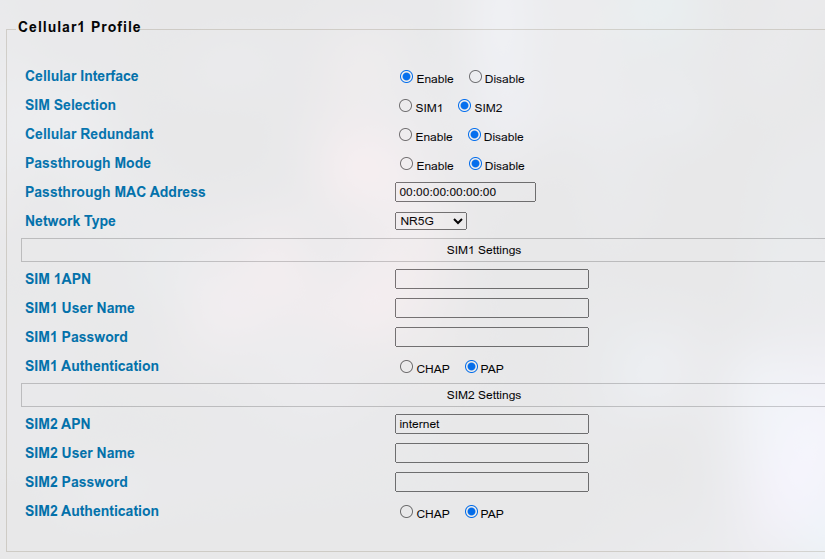
\includegraphics[width=0.6\textwidth]{02-cellular-settings-apn.png}
\caption{APN configurado no roteador.}
\end{figure}

Antes da correção do TAC, a UE permanecia não registrada e detectava apenas
a rede comercial \code{724 03}. Após a correção, registrou na primeira
tentativa (Figura~\ref{fig:ue}).

\begin{figure}[H]
\centering
\begin{minipage}{0.52\textwidth}\centering
  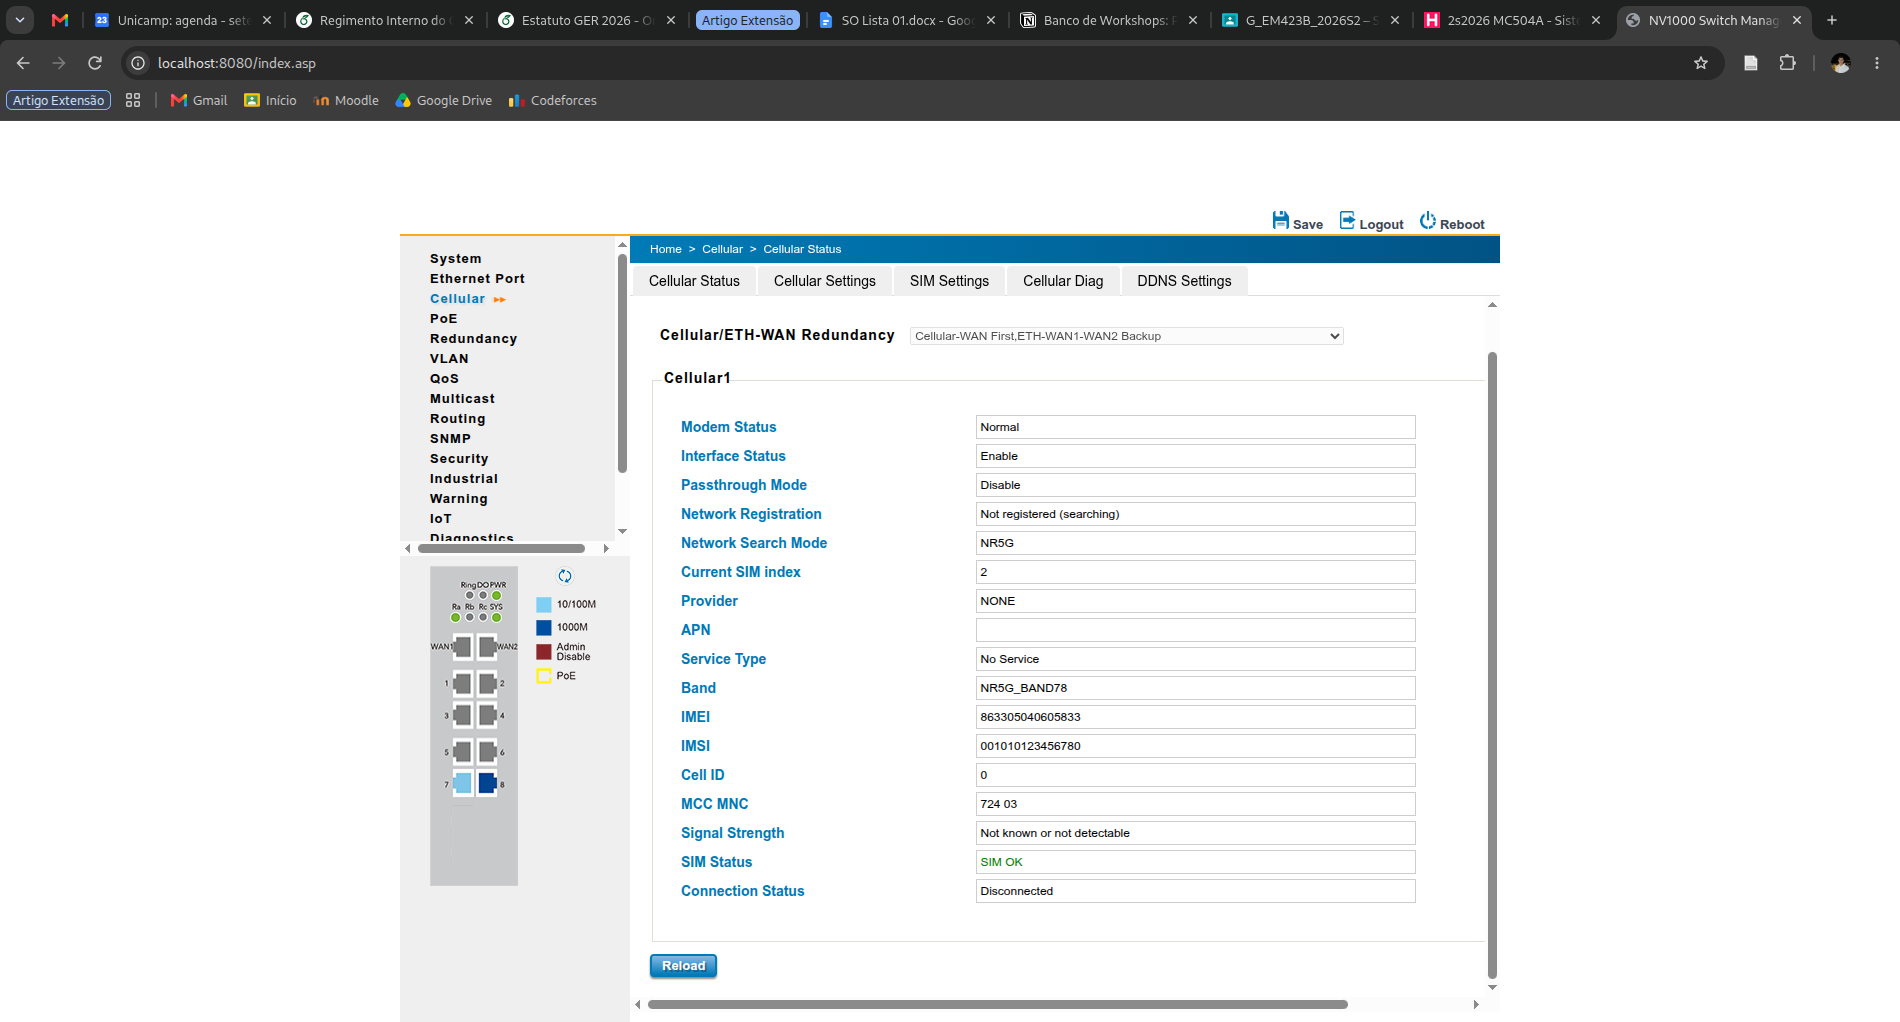
\includegraphics[width=\linewidth]{01-cellular-status-plmn-errado.png}\\
  \small (a) antes: não registrada
\end{minipage}\hfill
\begin{minipage}{0.42\textwidth}\centering
  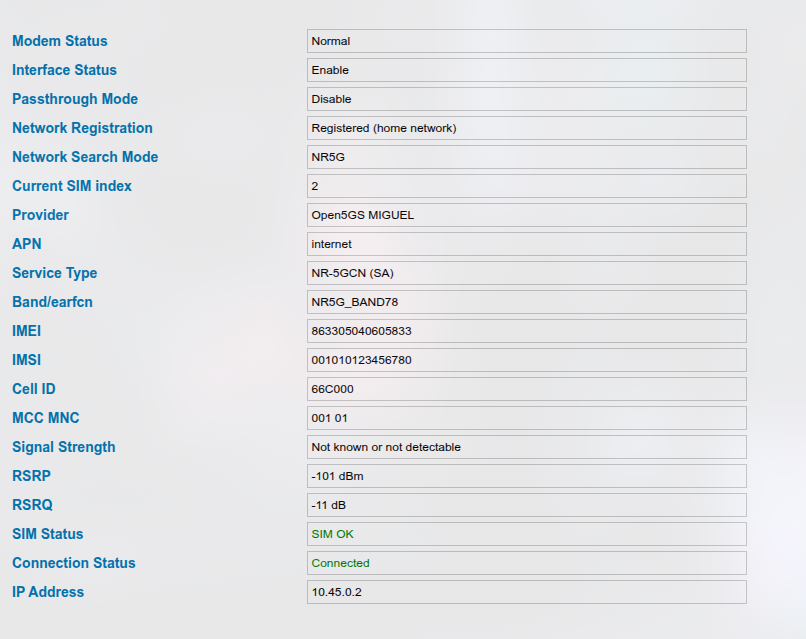
\includegraphics[width=\linewidth]{03-cellular-status-connected.png}\\
  \small (b) depois: registrada
\end{minipage}
\caption{Estado celular da UE.}
\label{fig:ue}
\end{figure}

\begin{table}[H]
\centering
\small
\begin{tabular}{@{}ll@{}}
\toprule
Registro & \emph{Registered (home network)} \\
Serviço & NR-5GCN (SA) \\
PLMN & 001 01 \\
RSRP / RSRQ & $-101$ dBm / $-11$ dB \\
IP atribuído & \code{10.45.0.2} (muda a cada reconexão) \\
\bottomrule
\end{tabular}
\caption{UE conectada.}
\end{table}

O sinal é fraco, porém funcional. O hub fica numa porta LAN (1--8). As portas
\code{wan1}/\code{wan2} servem de \emph{backup} e devem ficar desconectadas
durante os testes, pois o roteador pode migrar o tráfego para Ethernet sem
aviso e invalidar a comparação.

\begin{figure}[H]
\centering
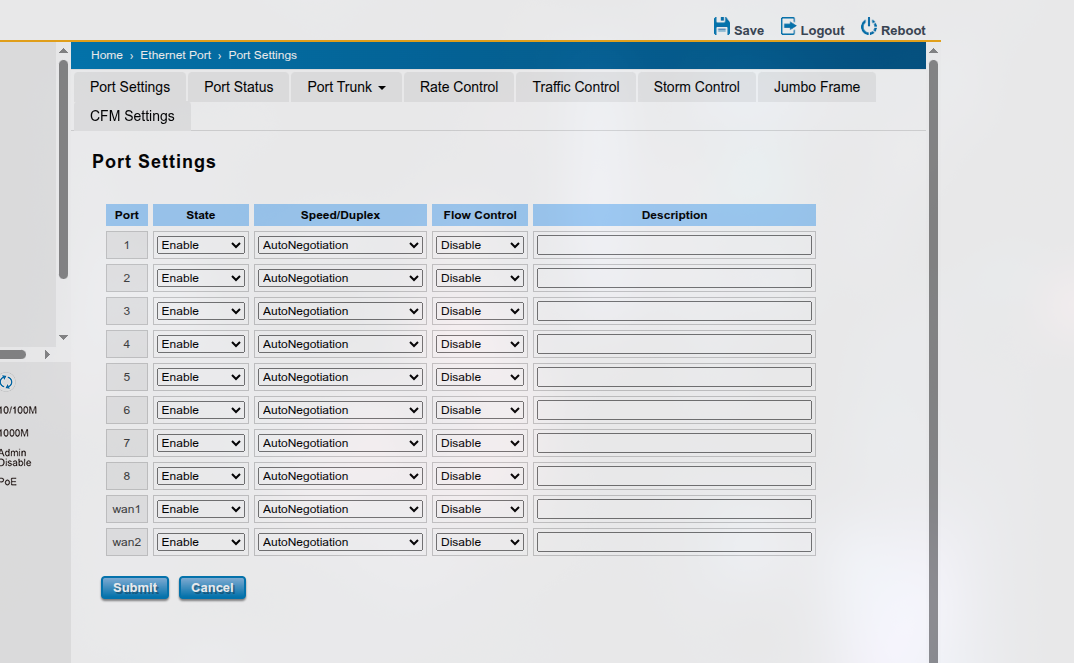
\includegraphics[width=0.7\textwidth]{04-ethernet-port-settings.png}
\caption{Mapa de portas Ethernet do roteador.}
\end{figure}

\section{Exposição do hub pela rede 5G}

Um cliente do lado do core precisa alcançar \code{192.168.10.250:502}
passando pelo roteador. A UE responde a \code{ping}, mas conexões TCP na
porta 502 não recebem resposta.

\begin{table}[H]
\centering
\small
\begin{tabularx}{\textwidth}{@{}lX@{}}
\toprule
Tentativa & Resultado \\
\midrule
\emph{Port forwarding} 502 $\to$ hub &
  SYN chega ao hub (\code{tcpdump} em \code{ogstun}), sem resposta. Outra regra
  (porta 80) retorna \code{No route to host}, logo o encaminhamento funciona. \\
NAT 1:1 &
  Mesmo mecanismo de DNAT; não concluída. \\
Modbus TCP Gateway do roteador &
  Descartada. O recurso torna o roteador um escravo Modbus próprio; não há
  campo de destino. \\
\emph{Hairpin NAT}/masquerade &
  Sem opção na interface web. Via \code{iptables} exigiria acesso SSH ao
  roteador, indisponível. \\
\bottomrule
\end{tabularx}
\caption{Tentativas de expor o hub.}
\end{table}

\begin{figure}[H]
\centering
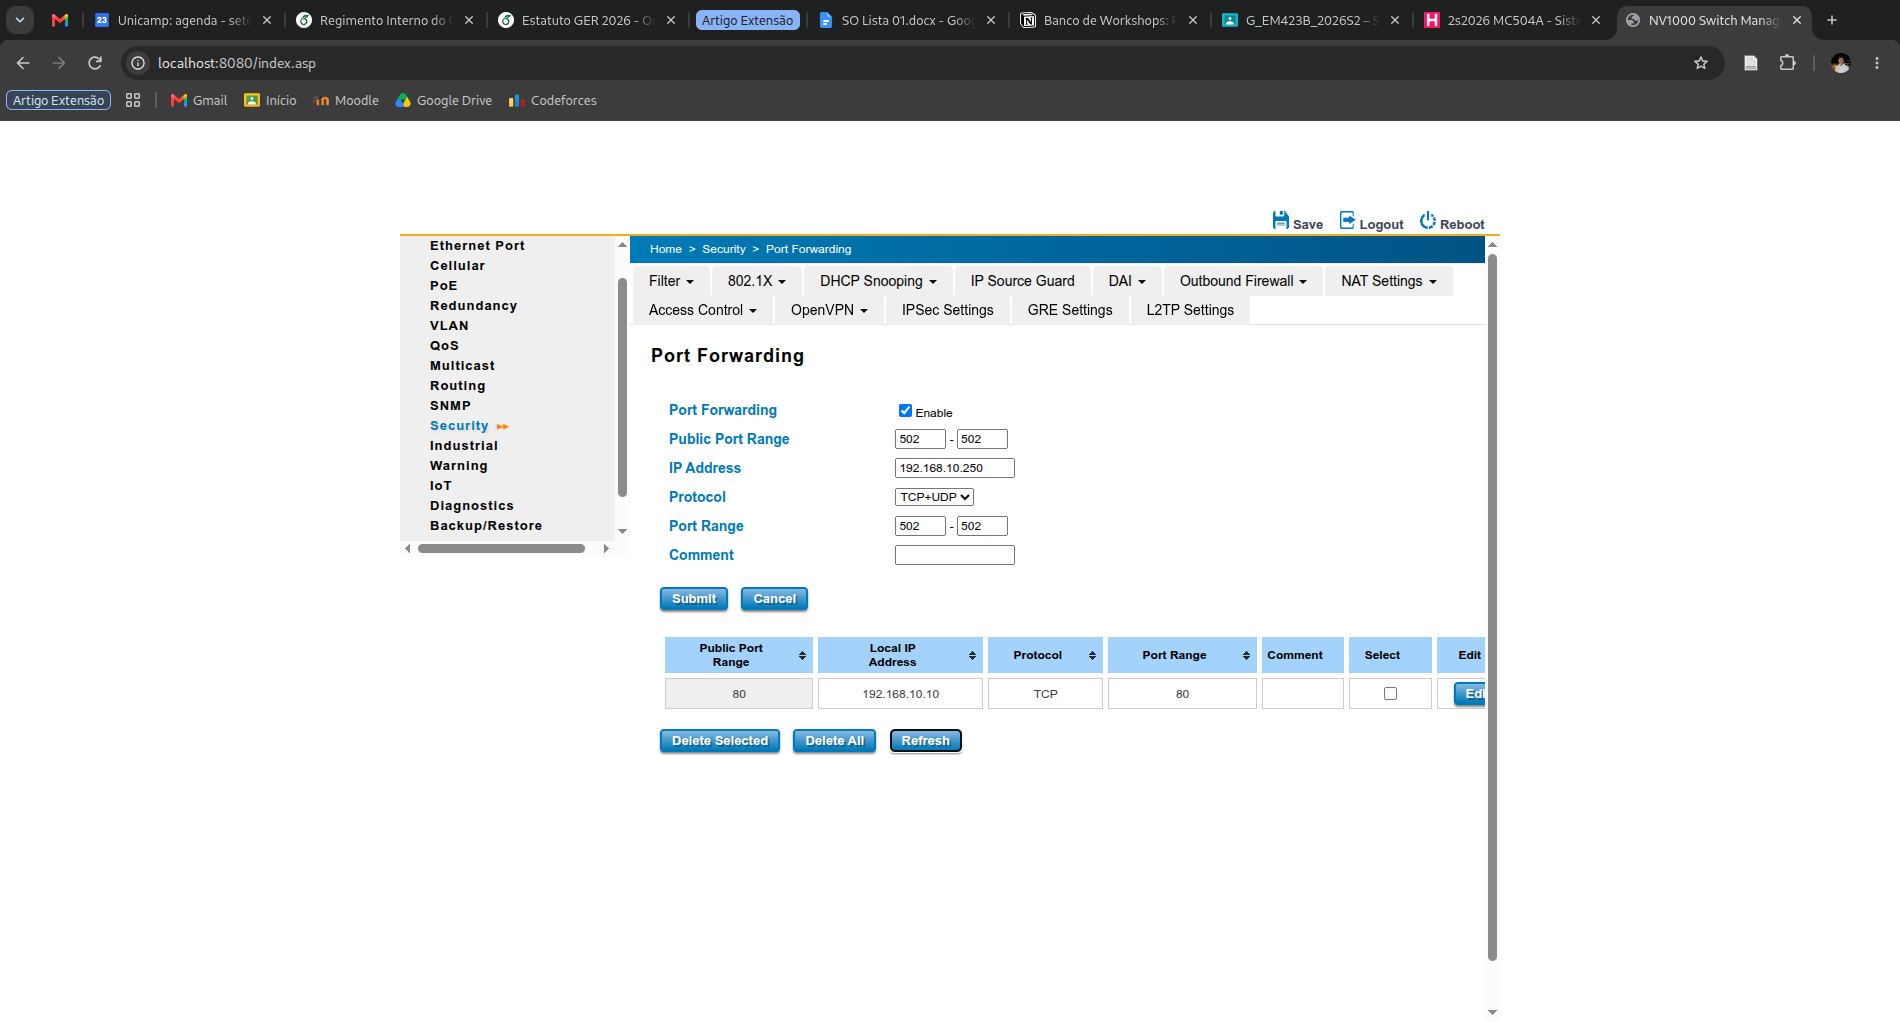
\includegraphics[width=0.65\textwidth]{06-port-forwarding.png}
\caption{Regra de \emph{port forwarding} 502 $\to$ \code{192.168.10.250:502}.}
\end{figure}

\paragraph{Causa.} O roteador faz DNAT sem alterar a origem: o hub recebe
pacotes de \code{10.45.0.x}, fora da sua sub-rede, e não tem
\emph{gateway} padrão configurado (\code{0.0.0.0} de fábrica) para responder.

\paragraph{Solução proposta.} Configurar \emph{default gateway}
\code{192.168.10.1} na porta \emph{fieldbus} do AL1340. Segundo o manual
(seção 9.1.6)~\cite{ifm-al1340-manual}, esse campo só é editável pelo LR DEVICE (software ifm) ou pela
API JSON da porta IoT (X23), nunca pela porta Modbus. O LR DEVICE é o caminho
indicado, pois alcança o hub pela rede já cabeada. A tentativa pela porta X23
falhou: o hub não foi descoberto em \code{169.254.0.0/16}. Em ambos os casos a
conexão Modbus deve estar encerrada durante a alteração. Chamada equivalente
pela API JSON:

\begin{lstlisting}
curl -X POST http://<IP_porta_IoT>/ -H "Content-Type: application/json" \
  -d '{"code":"request","cid":1,"adr":"/fieldbussetup/network/ipdefaultgateway/setdata","data":{"newvalue":"192.168.10.1"}}'
\end{lstlisting}

\section{Execução do bench}

Com o hub acessível pela 5G:

\begin{lstlisting}
make bench HOST=<IP da UE> PORT=502 LABEL=5g
make plot
ip route get 192.168.10.250   # confirma que o tráfego não sai pela LAN
\end{lstlisting}

Antes de cada execução, conferir o IP atual da UE e a rota usada pelo host.

\section{Problemas encontrados}

\begin{table}[H]
\centering
\small
\begin{tabularx}{\textwidth}{@{}XXX@{}}
\toprule
Sintoma & Causa & Correção \\
\midrule
\code{N2: Failed to connect to AMF} & \code{amf.yaml} sem bloco \code{ngap} & Adicionar \code{ngap.server} \\
\code{unknown-PLMN-or-SNPN} & TAC da gNB $\neq$ TAC do AMF & Igualar TAC \\
\code{Could not find cell PLMN \ldots} & TAC divergente dentro da config da gNB & Igualar TAC \\
\code{exceeds the maximum capacity} & USRP em USB~2 & Usar USB~3 ou banda de 10~MHz \\
UE não registrada, PLMN comercial & NG Setup rejeitado & Corrigir TAC \\
Porta 502 sem resposta via 5G & Hub sem \emph{gateway} padrão & Configurar \emph{gateway} via LR DEVICE \\
\code{address already in use} (9999) & WebUI nativa e Docker na mesma porta & Manter apenas a nativa \\
\bottomrule
\end{tabularx}
\caption{Resumo de problemas e correções.}
\end{table}

\section{Situação atual e próximos passos}

\begin{itemize}
  \item Acesso Modbus local ao hub: validado.
  \item Rede 5G SA (core, gNB, UE): operacional, UE registrada com PLMN 00101.
  \item Acesso ao hub através da 5G: causa identificada; pendente configurar o
    \emph{gateway} do hub e validar o \emph{port forwarding}.
  \item Medição de latência sobre 5G: aguardando o item anterior.
  \item \emph{Network slicing}: configurações preparadas em \code{5g-slicing/}
    (Open5GS + UERANSIM, ambiente simulado); falta aplicá-las à rede com rádio
    real e medir o efeito sobre a latência do bench.
\end{itemize}

\begin{thebibliography}{99}
\small

\bibitem{ifm-al1340-manual}
ifm electronic.
\newblock \emph{Operating Instructions: IO-Link Master with Modbus TCP
  Interface DataLine 4 Ports, AL1340}.
\newblock Doc. 80284126/01, firmware 2.3.x, set. 2019.

\bibitem{ifm-al1340}
ifm electronic.
\newblock AL1340 --- IO-Link master with Modbus TCP interface (página do produto).
\newblock \url{https://www.ifm.com/us/en/product/AL1340}

\bibitem{ifm-modbus-notes}
ifm electronic.
\newblock \emph{Modbus basic setup notes for IO-Link AL1xxx Master Block}.
\newblock \url{https://www.ifm.com/binaries/content/assets/us/pdfs/io-link-support/9129_modbus_web_update__v2.pdf}

\bibitem{hms-nv1000}
HMS Networks.
\newblock Anybus Wireless Router 5G (NV1000) (página do produto).
\newblock \url{https://www.hms-networks.com/p/nv1000-wireless-router-5g}

\bibitem{modbus}
Modbus Organization.
\newblock \emph{MODBUS Application Protocol Specification V1.1b3}.
\newblock \url{https://www.modbus.org/modbus-specifications}

\bibitem{pymodbustcp}
L. Lefebvre.
\newblock pyModbusTCP: a simple Modbus/TCP client/server library for Python.
\newblock \url{https://github.com/sourceperl/pyModbusTCP} ---
  documentação: \url{https://pymodbustcp.readthedocs.io}

\bibitem{pymodbus}
Pymodbus.
\newblock Pymodbus: a full Modbus protocol implementation in Python.
\newblock \url{https://pymodbus.readthedocs.io}

\bibitem{mbpoll}
P. Jean.
\newblock mbpoll: command line utility to communicate with Modbus slaves.
\newblock \url{https://github.com/epsilonrt/mbpoll}

\bibitem{flask-socketio}
M. Grinberg.
\newblock Flask-SocketIO.
\newblock \url{https://flask-socketio.readthedocs.io}

\bibitem{open5gs}
Open5GS.
\newblock Open5GS documentation.
\newblock \url{https://open5gs.org/open5gs/docs/}

\bibitem{srsran}
SRS.
\newblock srsRAN Project documentation.
\newblock \url{https://docs.srsran.com/projects/project/en/latest/}

\bibitem{uhd}
Ettus Research.
\newblock USRP Hardware Driver (UHD) manual.
\newblock \url{https://files.ettus.com/manual/}

\end{thebibliography}

\end{document}
